\label{sec:CRLFR}
The measurement of the lepton fake rate, which is the probability that a fake lepton that passes the loose selection also passes the tight criteria,
is carried out in a separate control region which is enriched in contempt leptons.

This region, denoted as $\PZ+L$, is defined as containing a valid \PZ candidate whose leptons must have $\pt^{\Pl_{Z,1}} > 20 \GeV$ and $\pt^{\Pl_{Z,2}} > 10 \GeV$
and an additional lepton which passes the loose selection.
Additionally, the \PZ candidate must have a mass within 10\GeV from the nominal peak,
and the missing energy must be $\MET < 20 \GeV$ to reduce the contribution from real leptons from $\PW\PZ$.
The last requirement means that this region is orthogonal to all of the regions in the 3\Pl channel, in which the MET is required to be greater than 30\GeV.

The fake rate is measured on the third lepton in several bins of transverse momentum, separately for the barrel and endcap and flavour.
The measurement is done for each year of data taking, and the resulting rates can be seen in Figure \ref{fig:leptonFR}.

\begin{figure}
  \centering
  \subfigure [2016] {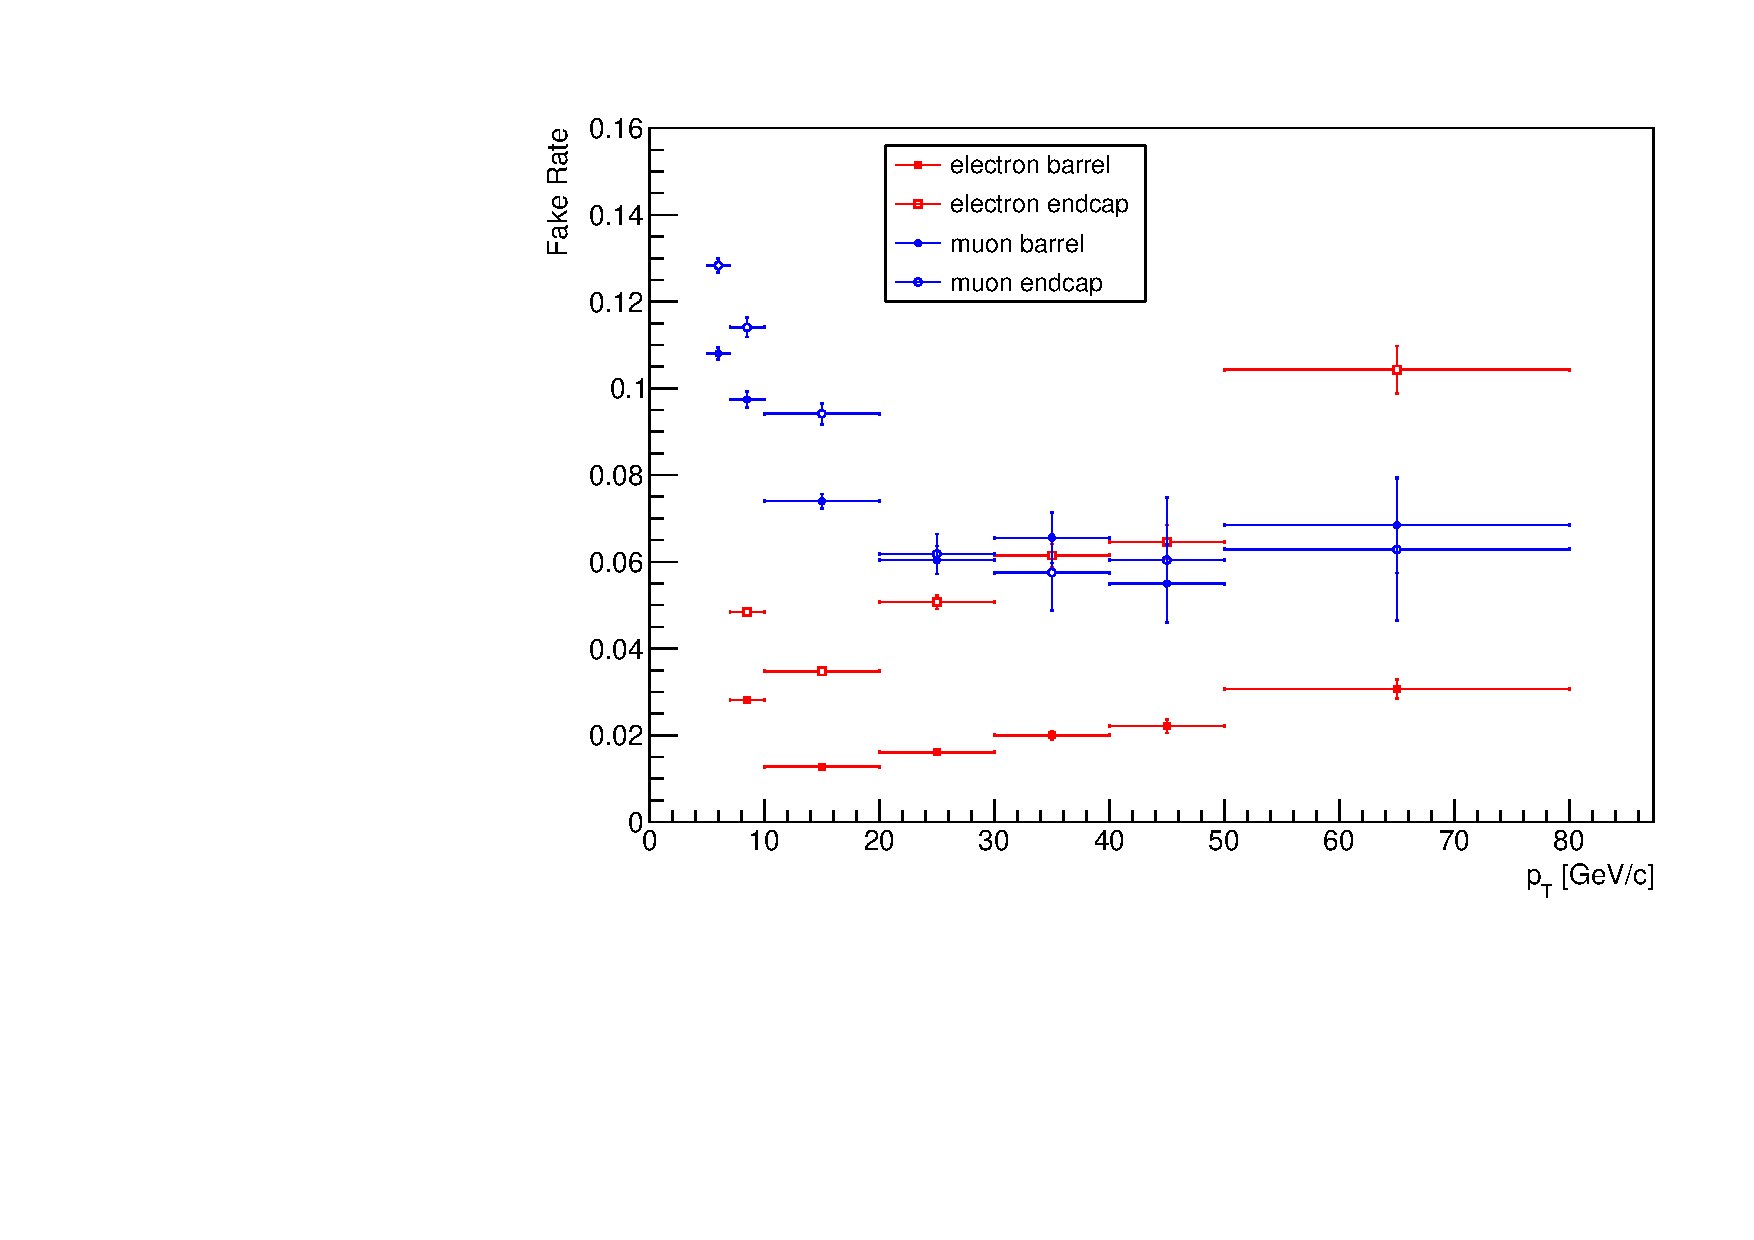
\includegraphics[width=.5\textwidth]{leptonFakeRate_2016.pdf}}%
  \subfigure [2017] {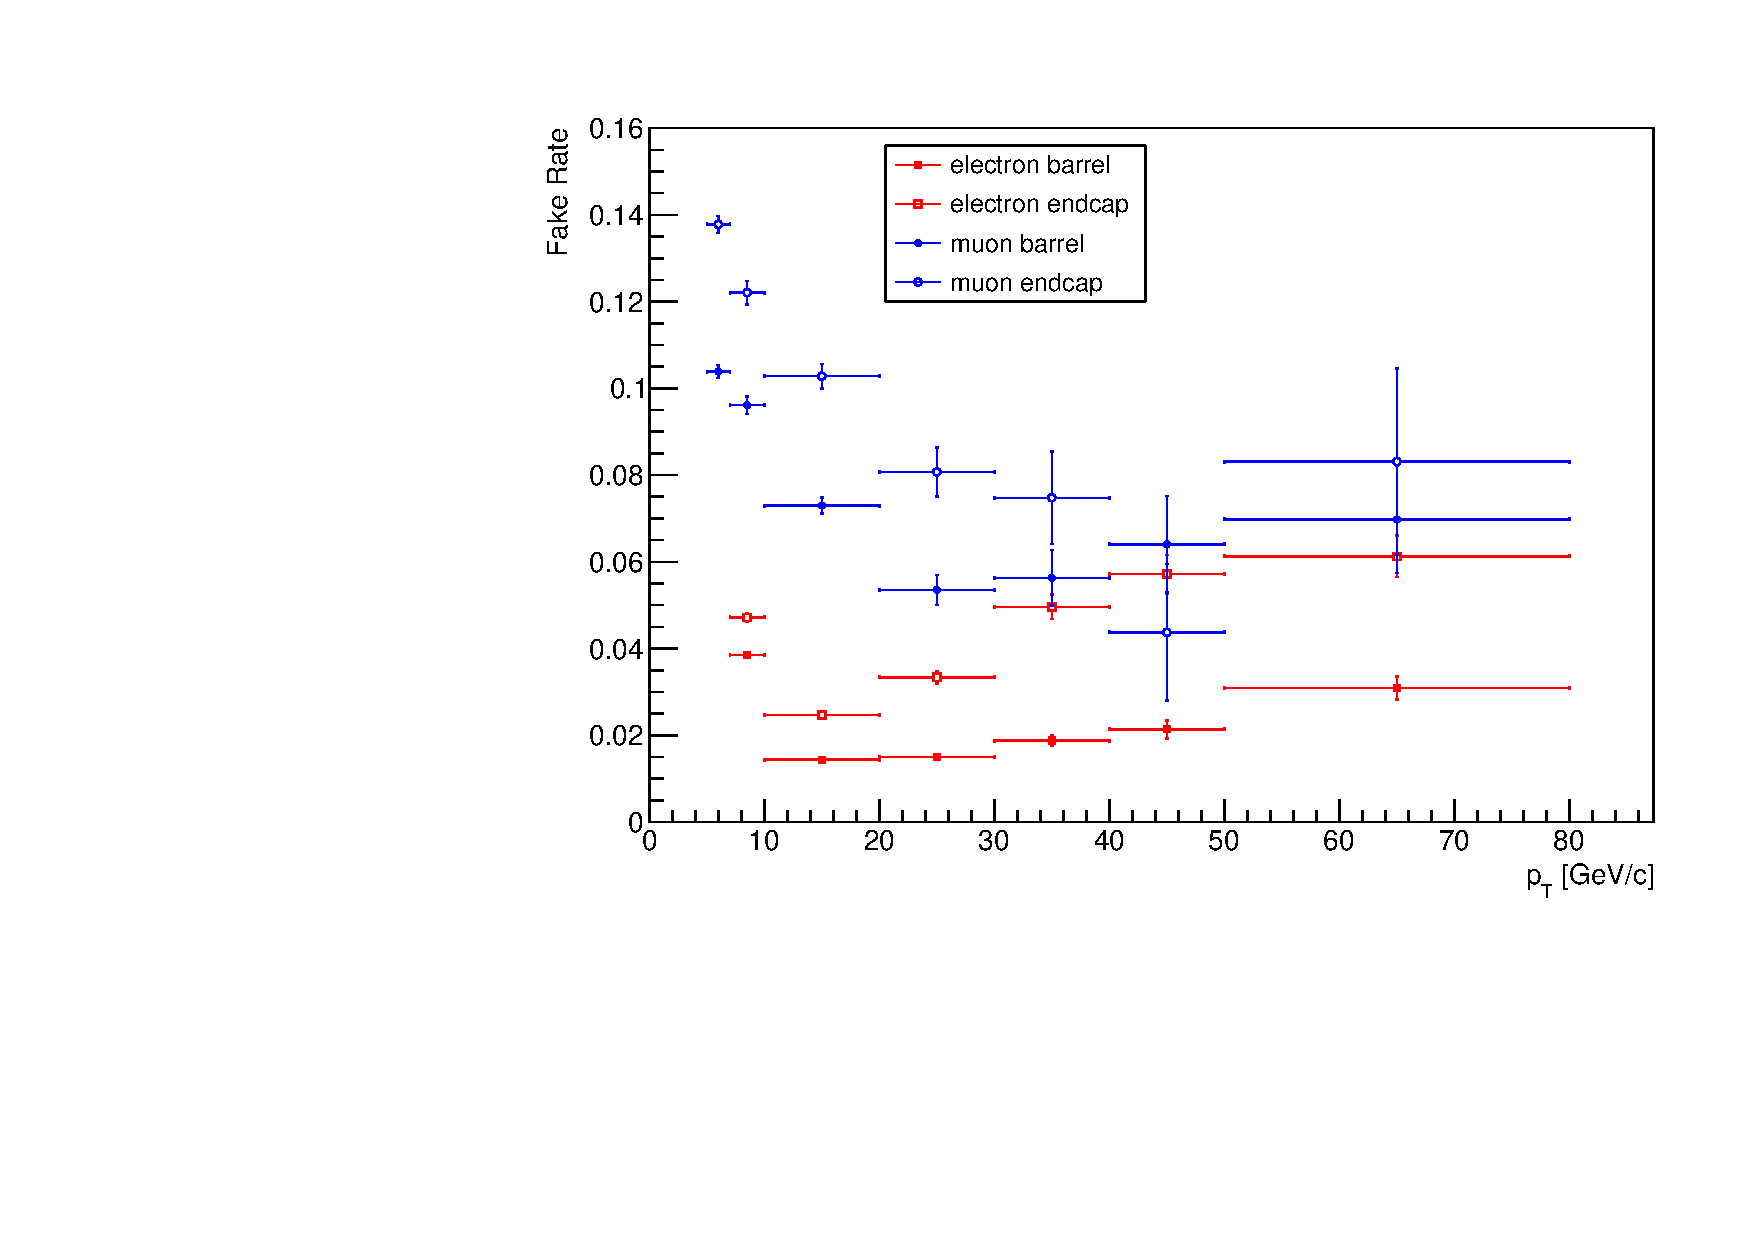
\includegraphics[width=.5\textwidth]{leptonFakeRate_2017.pdf}}\\
  \subfigure [2018] {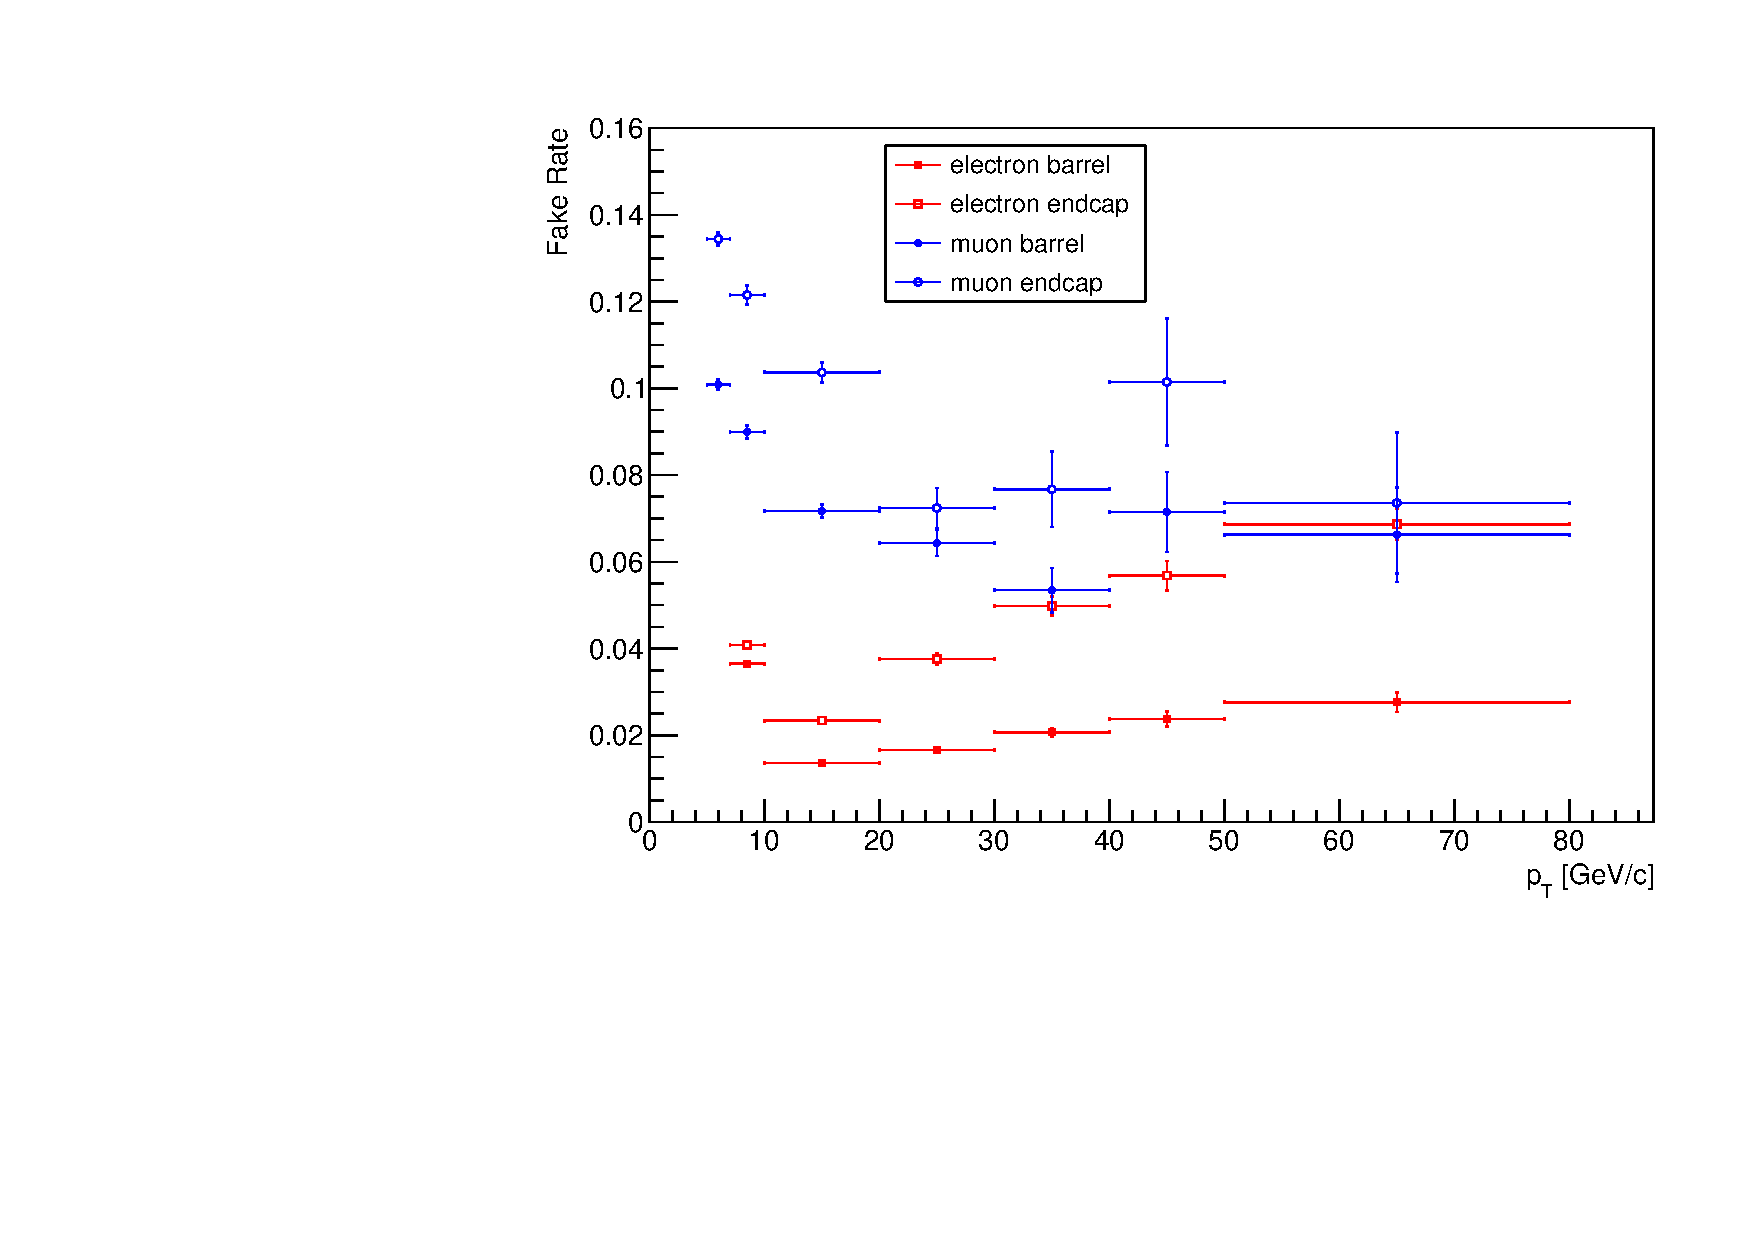
\includegraphics[width=.5\textwidth]{leptonFakeRate_2018.pdf}}
  \caption{Lepton fake rates measured in the $\PZ+L$ control region, for each year of data-taking.}
  \label{fig:leptonFR}
\end{figure}

The main uncertainty on the fake lepton background estimation arises from
the limited statistics in the application regions,
for the four lepton channel in particular,
and in the fake rate measurement region.
An additional uncertainty is due to the difference in composition of the
background processes in the region where the fake rate is measured and where it is applied.
The uncertainty was measured by several analyses and found to be
20\usep\%, 25\usep\%, and 40\usep\% for the $4\Pe$, $2\Pe2\PGm$, and $4\PGm$ decay channels,
respectively~\cite{CMS-HIG-13-002}.
Others reported a flat 40\usep\% uncertainty~\cite{CMS-SMP-20-001,CMS-PAS-SMP-22-001}.
